\chapter{Modellizzazione f{}isica del LINAC nel TPS RayStation}
\minitoc
\textsf{In questo capitolo verranno introdotti i concetti di dosimetria di base di un acceleratore lineare. A partire da queste misure, viene costruito un modello dosimetrico del LINAC all'interno del TPS. Viene poi discussa l'accuratezza richiesta per un calcolo dosimetrico al variare della tecnica di erogazione assieme alle scelte e i metodi adottati per raggiungerla.}



\section{Dosimetria di base di un LINAC}
Le misure necessarie a costruire un modello dosimetrico di un LINAC consistono in curve di dosimetria relativa e misure puntuali di dose (assoluta e relativa).\\
Storicamente queste misurazioni vengono effettuate con detector a camera a ionizzazione. Tuttavia, con l'avvento delle tecniche di radioterapia avanzata (es. intensità modulata o stereotassi) sono stati introdotti una molteplicità di detector di nuova generazione per soddisfare le esigenze di accuratezza di misura per piccoli campi di irradiazione\footnote{Un campo quadrato è ritenuto \textit{piccolo} se inferiore a $4$x$4$ cm$^2$ \cite{Das2008}.}. Nella sezione seguente verranno presentati i concetti classici di dosimetria di un LINAC propedeutici alla modellizzazione di un TPS. Ci si soffermerà dapprima alla tecnica di irradiazione denominata \textit{radioterapia conformazionale}\footnote{La radioterapia conformazionale o 3D-CRT è una tecnica di irradiazione che  fa impiego di fasci di irradiazione collimati sul target per i quali la pianificazione ed il calcolo della dose vengono effettuati su uno studio di tomografia computerizzata del paziente.}. Le problematiche relative alla dosimetria a piccoli campi e alle tecniche di irradiazione avanzata verranno discusse a seguire. 

\subsection{Dosimetria relativa}
Per dosimetria relativa si intende tutta una serie di misure della dose non in termini assoluti (in Gray) ma in percentuale rispetto a uno o più riferimenti. In particolare le misure necessarie alla modellizzazione in genere di un TPS possono essere suddivise in tre catagorie:
\begin{itemize}
\item Curve di dose-profondità (PDD).
\item Profili di dose.
\item Output factor.
\end{itemize}
Queste misure vengono effettuate in un fantoccio cubico riempito di acqua (materiale più simile ai tessuti umani) dotato di un carrello motorizzato su cui viene montata la camera a ionizzazione che effettua le misure di dose (vedi Fig.\ref{fig:wphant}).
\begin{figure}
\centering
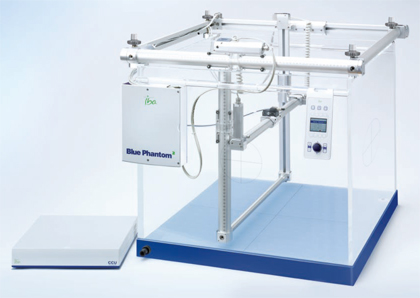
\includegraphics[width=.47\textwidth]{./cap2/wphant.jpg}
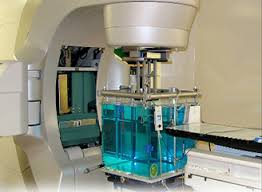
\includegraphics[width=.47\textwidth]{./cap2/wphant_pos.jpg}
\caption{Fantoccio per le misure di dosimetria assoluta e relativa (foto e suo posizionamento rispetto al LINAC).}
\label{fig:wphant}
\end{figure}

Le curve di dose-profondità si ottengono muovendo il detector lungo l'asse centrale del fascio (in direzione verticale) con un certo step (tipicamente 1 mm).\\
Per ogni punto, la camera a ionizzazione registra una certa dose che viene normalizzata rispetto ad una lettura di riferimento (tipicamente la lettura corrispondente alla massima dose lungo la verticale).

I profili di dose si ottengono in maniera analoga muovendo il detector in piani perpendicolari all'asse del fascio. Tipicamente vengono acquisiti profili di dose lungo due assi perpendicolari denominati \textit{inline} e \textit{crossline}\footnote{Considerando un paziente supino con la testa verso il gantry del LINAC, l'asse \textit{inline} corrisponde alla direzione testa-piedi e l'asse \textit{cross-line} alla direzione sinistra-destra.} a varie profondità.\\
\begin{figure}
\centering
\includegraphics[width=\textwidth]{}
\caption{}
\label{fig:pdd_prof}
\end{figure}
Nella Fig.\ref{fig:pdd_prof} è possibile visualizzare l'andamento tipico di una curva dose-profondità e di un profilo di dose.

Nelle curve di dose-profondità è possibile distinguere due zone:
\begin{itemize}
\item \textit{zona di build-up:} la prima parte ascendente della PDD in cui viene 
\end{itemize}

Una estensiva review dei detector e delle tecniche di misura consigliate per piccoli campi è stata recentemente pubblicata dal task group 120 dell'associazione americana dei fisici medici (AAPM) \cite{Low2011}.




